%% Intended to be included into a larger document
\chapter{Related Work}

%% Add more to introduce topics in this chapter?

\section{Does Energy Efficiency Reduce Carbon Emissions?}
\label{sec:efficiency-rebound}

Many governmental plans to reduce GHG emissions involve improving energy efficiency in the home, in industry, and in transportation. While intuitively it would seem that increased energy efficiency would lead to decreased energy usage, and thereby reduced GHG emissions, surprisingly there is some evidence (both theoretical and empirical) that energy efficiency actually increases energy usage! Saunders dubbed this unintuitive notion the Khazzoom-Brookes Postulate based on conclusions reached independently by those two researchers \cite{saunders-1992}. \fxnote{Insert references to Khazzoom and Lovins papers here, after I read them.}

Using neoclassical growth theory, Saunders finds that increased energy efficiency makes energy seem cheaper, thus allowing it to be substituted for labor in production. Increased energy efficiency also increases overall economic growth, which leads to increased overall energy usage.

In discussing this effect, rebound is defined as the difference between the expected amount of energy savings from an improvement in energy efficiency, and the actual observed effect. For example, if an improvement in metal smelting technology reduces the energy required to smelt by 20\%, but the energy consumed by the metal smelting industry only goes down by 10\% then the rebound is 50\%. If the rebound is greater than 100\%, then backfire is taking place (the efficiency measure has backfired) \cite{Hanley2008Do-increases-in}. There is some debate over whether the predicted increases in energy usage will actually take place in the real world. Laitner suggests via a simple analysis that the rebound effect is small (2.4\%) \cite{Skip-Laitner:2000yg}. His equation relates future carbon emissions to current carbon emissions, increases in GDP and energy costs, and elasticities of income and energy prices to arrive at this conclusion. He goes on to a further analysis done by the Environmental Protection Agency and Lawrence Berkeley National Labs using the National Energy Modeling System showing that an ``energy-efficient/low-carbon technology path'' would suffer from a rebound effect of only 2.2\%. However, he acknowledges that consumer choices about energy usage could erode gains from efficiency, such as turning up the furnace thermostat because the cost of doing so has been effectively reduced.

The issue of consumer choices is a real one. Over the last 25 years, automobiles have been made more efficient through ``increasing the efficiency of the engine and transmission, decreasing weight, improving tires and reducing drag'' \cite{Heywood2008Fueling-Our-Future}. However, these improvements have been traded for vehicles that are larger, heavier, and faster, which has led to only modest improvements in overall fuel efficiency. This is an example of how energy efficiency may not always lead to reduced GHG emissions without motivating automobile users (and manufacturers) to buy and make fuel efficient vehicles.

Other authors find that rebound and even backfire are the likely results of economy-wide improvements in energy efficiency. The analysis of Hanley et al. finds that backfire occurs when economy-wide improvements in energy efficiency are made \cite{Hanley2008Do-increases-in}. Their theoretical analysis finds that if energy demand is relatively price-elastic (demand increases when prices are low and decreases when prices are high), then backfire will occur. Empirical evidence of rebound and backfire are hard to come by because there are indirect system-wide effects due to the increased efficiency, and these indirect effects are difficult to measure. The authors created a Computable General Equilibrium (CGE) model of Scotland that simulates the economy and environmental impact based on the inputs and outputs of the system. Using this model, almost all scenarios eventually result in backfire. They note that since non-renewable energy sources use more energy in their production than renewable sources, increased energy efficiency lowers the cost of non-renewables compared to renewables, financially favoring the use of non-renewables. Efficiency in energy production is therefore associated with a decrease in the use of energy from renewable sources. The authors also urge caution when reviewing sustainability measures such as the ratio of Gross Domestic Product (GDP) to energy usage or carbon emissions, because even if the ratio increases (less carbon per unit GDP), if the GDP as a whole increases faster, the absolute carbon emitted will increase. They suggest that backfire could be prevented by combining energy efficiency improvements with taxes on energy use or a carbon tax. Since energy efficiency effectively reduces the cost of energy, the savings could offset the cost of additional taxes, thereby blunting any impact on economic activity.

It would appear that any energy efficiency improvements will have some degree of rebound effect, thus a naive pursuit of energy efficiency without taking into account the context around the improvements could risk reducing their effectiveness, or even making them counterproductive! While many of the analyses deal at the macroeconomic level, it is not hard to think of individual scenarios where efficiency could actually increase personal usage, such buying two energy efficient refrigerators to replace one older energy-hogging refrigerator. The key to ensuring that energy efficiency improvements on the micro level lead to less GHG emissions is to combine efficiencies with changes in behavior.

\section{Energy Feedback}
\label{sec:energy-feedback}

To reduce energy use, people must know how much energy they are is using. Feedback systems display the consumption of a resource (such as electricity) to the user, usually in real time. Darby provides a detailed survey of studies on electricity feedback systems from the past 3 decades \cite{darby-review-2006}. The survey of 20 studies finds that, on average, the introduction of a direct (real-time) feedback system leads to reductions of energy usage ranging from 5-15\%. Feedback systems providing historical data (such as those provided with billing statements) are not as effective (0-10\% reductions), but can be useful for assessing the impact of efficiency measures such as improved insulation or a more energy efficient appliance, since those savings accumulate over time.

Darby found that ``consumption in identical homes, even those designed to be low-energy dwellings, can easily differ by a factor of two or more depending on the behaviour of the inhabitants.'' This finding demonstrates the significant potential to curb energy usage through changes in individual's behavior.

\begin{figure}[htbp]
	\centering
		\includegraphics[scale=0.59]{current-energy-website}
		\caption{View of LBNL's Current Energy Web Site on December 15, 2004}
		\label{fig:current-energy-website}
\end{figure}

During California's energy crisis in 2000 and 2001, Lawrence Berkeley National Laboratory created a web site that graphed data from utility organizations \cite{Bartholomew2008Current-Energy}. The graphs showed consumer demand for electricity (actual and forecast), and the utilities' generation capacity (see \autoref{fig:current-energy-website} for an example graph). Darby reports anecdotal evidence that people viewing the graphs changed their electricity usage based on the data \cite{darby-review-2006}.

There is also evidence that just the knowledge that one is being monitored can cause one to consume fewer resources. A group of researchers simulating a mission to Mars or the Moon in the Canadian Arctic for four months tracked the crew members' water usage \cite{Bamsey2008FMARS}. Water usage was monitored via automated meters during the entire mission, but during certain multi-day study periods, crew members were also required to manually log their water usage at the point of use. The authors found that water usage was 10\% less during these study periods. The reduced water usage could be due to the knowledge that the usage was being examined more closely, or perhaps the extra effort required to manually record their water usage led to crew members reducing non-essential water use (see \autoref{sec:ecoisland} for another possible benefit to manual data collection).

While feedback can increase energy conservation, there are still cultural norms that strongly influence what behaviors are non-negotiable. Strengers performed an ethnographic study of 10 households participating in a smart metering trial to examine how their comfort and cleanliness norms affected their energy savings \cite{strengers-comfort-norms-2008}. Participants were provided with metering devices that displayed electricity and water usage, and greenhouse gas emissions in real time. The author was attempting to use feedback to change the participants societal norms for comfort and cleanliness. For example, until relatively recently, bathing weekly was the norm, but now bathing daily is considered normal behavior. Like many people, the participants did not understand the connection between the consumption data and their practices. Participants tended to increase conservation by changing technology (such as using compact florescent lamps (CFLs) instead of incandescent light bulbs), or by minor behavioral changes like ``taking shorter showers, doing full loads of laundry''.

Strengers states that people act the way they do (in matters of cleanliness and comfort) because ``they believe society expects them to'' and because many companies and organizations have a vested interest in keeping it that way. Therefore, just providing people information about their consumption is not enough, because individuals are constrained by infrastructures and social norms. She suggests increasing social interaction regarding the feedback system by making placement more prominent and encouraging discussion with household visitors, because people tend to conform to the expectations of their peers.
However, it would seem that changing societal norms is one of the hardest possible means for reducing consumption. It also feeds into many of the negative stereotypes of environmentalism: smelly people living in dark, cold homes. Despite the irrationality of some of these norms, effort may be better spent focusing on areas where the effort will meet less resistance.

\begin{figure}[htbp]
	\centering
		\subfigure[Device itself]{\label{fig:thighmaster-device}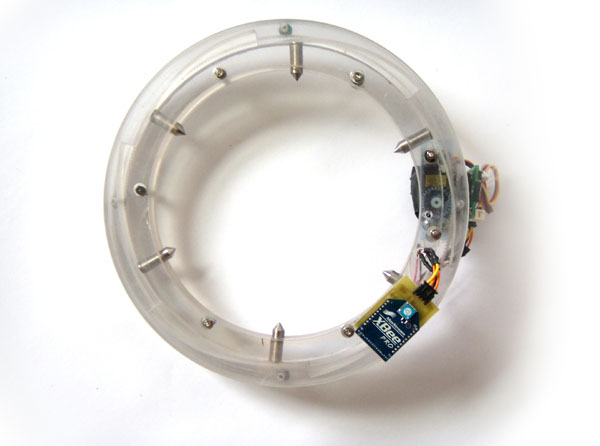
\includegraphics[height=2.5in]{thighmaster-alone}}
		\subfigure[As worn on leg]{\label{fig:thighmaster-leg}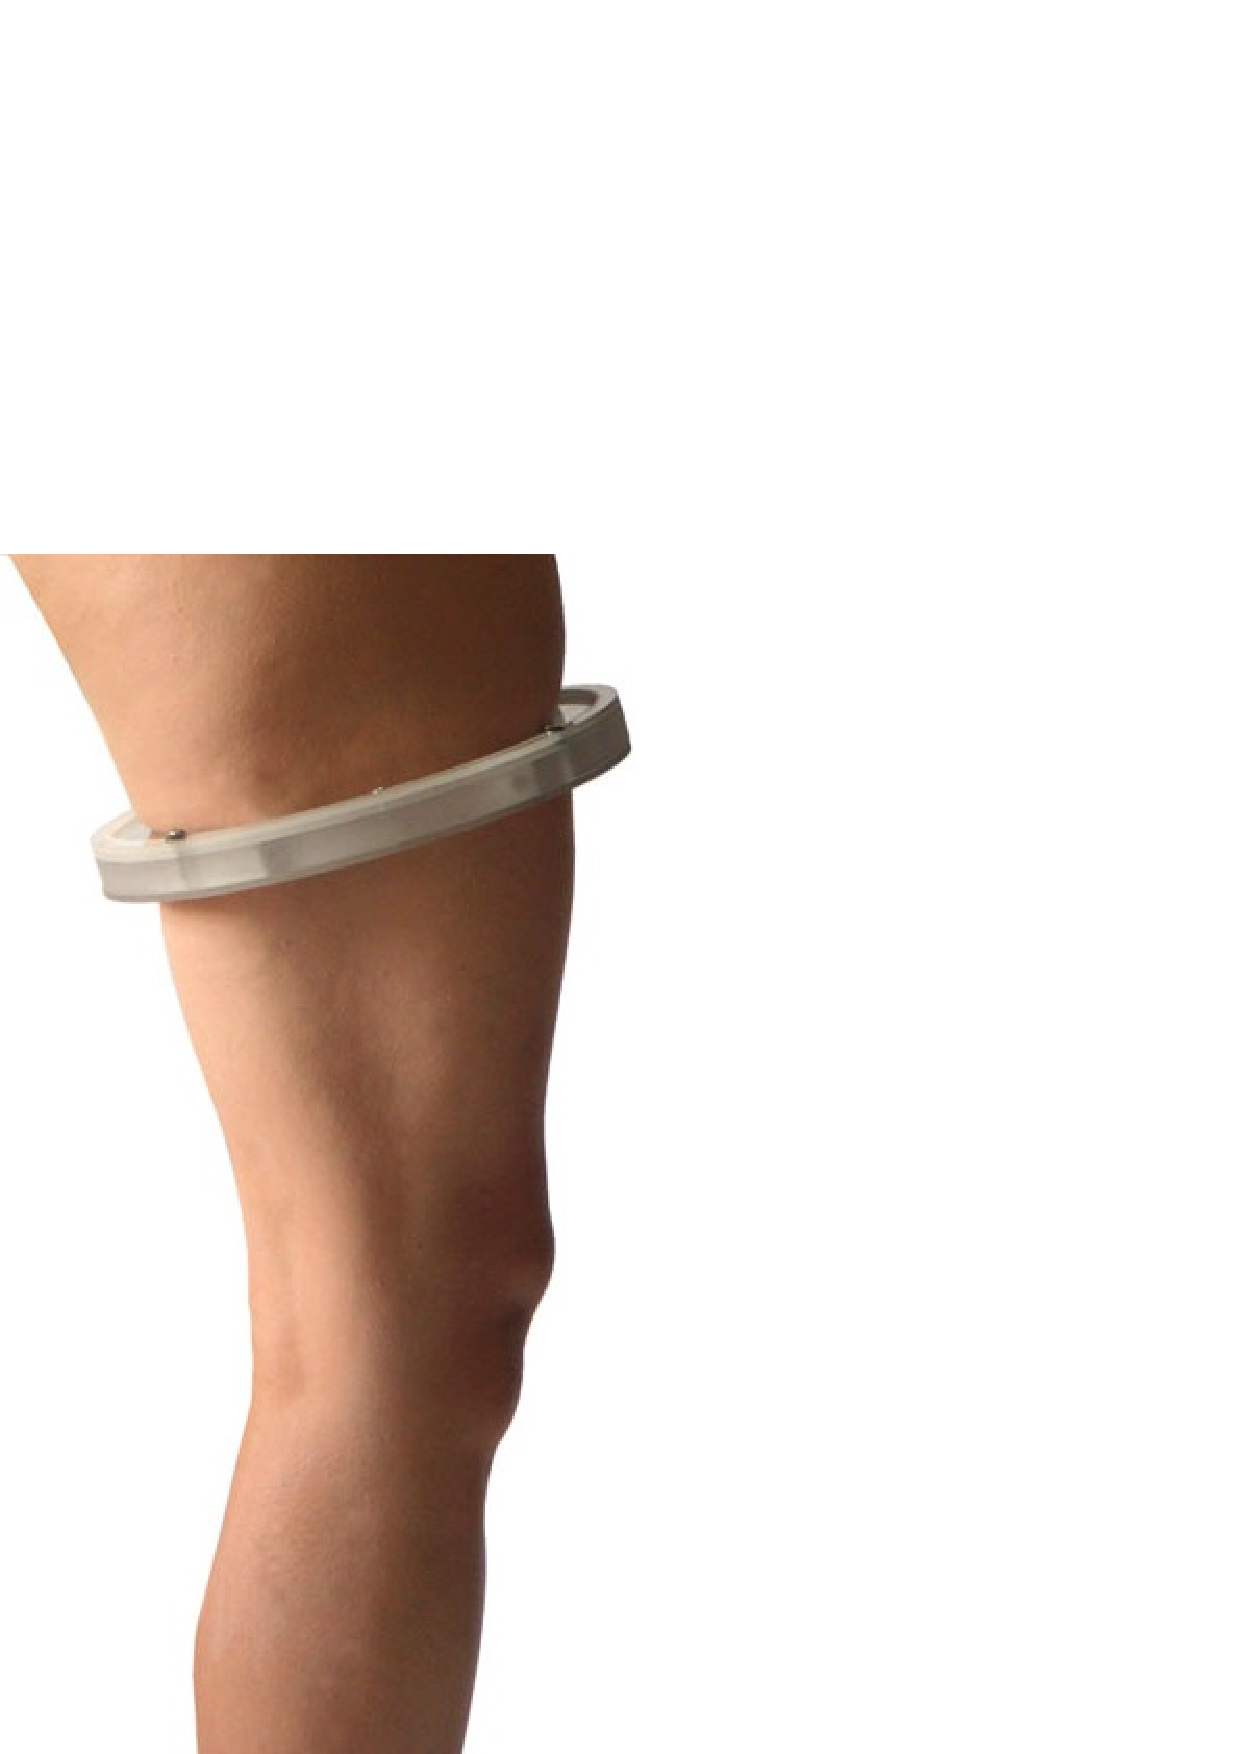
\includegraphics[height=2.5in]{thighmaster-leg}}
		\caption{Thighmaster energy feedback mortification device}
		\label{fig:thighmaster}
\end{figure}

R\"{u}st has implemented an extreme energy feedback system called the Thighmaster \cite{Rust2008Thighmaster-web}. Inspired by the cilice (a small metal garter with inward facing spikes) worn by some members of the Catholic Opus Dei organization as part of a practice of mortification, the Thighmaster is a ``techno-garter'' that pokes the wearer with spikes when their actions are not environmentally responsible (as defined by R\"{u}st), see \autoref{fig:thighmaster} for a depiction of the device. Specifically, the Thighmaster communicates wirelessly with electricity usage sensors and a human speech sensor that monitors whether the user speaks with their plants. While more of a demonstration, the Thighmaster shows the complex emotions involved in people's reactions to climate change. It goes without saying that being pierced by spikes is unlikely to be a viable energy feedback mechanism for most users.

\section{Dorm Energy Competitions}
\label{sec:dorm-energy-competitions}

\section{Related Systems}
\label{sec:related-systems}

In this section we examine other systems that have been designed to help users become more aware of their environmental impact.

\subsection{StepGreen}

\subsection{Personal Kyoto}

\subsection{EcoIsland}
\label{sec:ecoisland}

Takayama and Lehdonvirta have constructed a system they call EcoIsland, which attempts to ``motivate behaviour changes that reduce CO2 emissions'' using a background game-like activity, with a centrally installed display in the home \cite{takayama-2008}. \autoref{fig:ecoisland} shows an example of the user interface. Each family member has an avatar on the virtual island, and they set a family \COtwo emissions target. The family's emissions are tracked via sensors and self-reporting. If the emissions exceed the chosen target level, the water level on the island rises, and if the water level continues to rise it will eventually end the game.

\begin{figure}[htb]
	\centering
		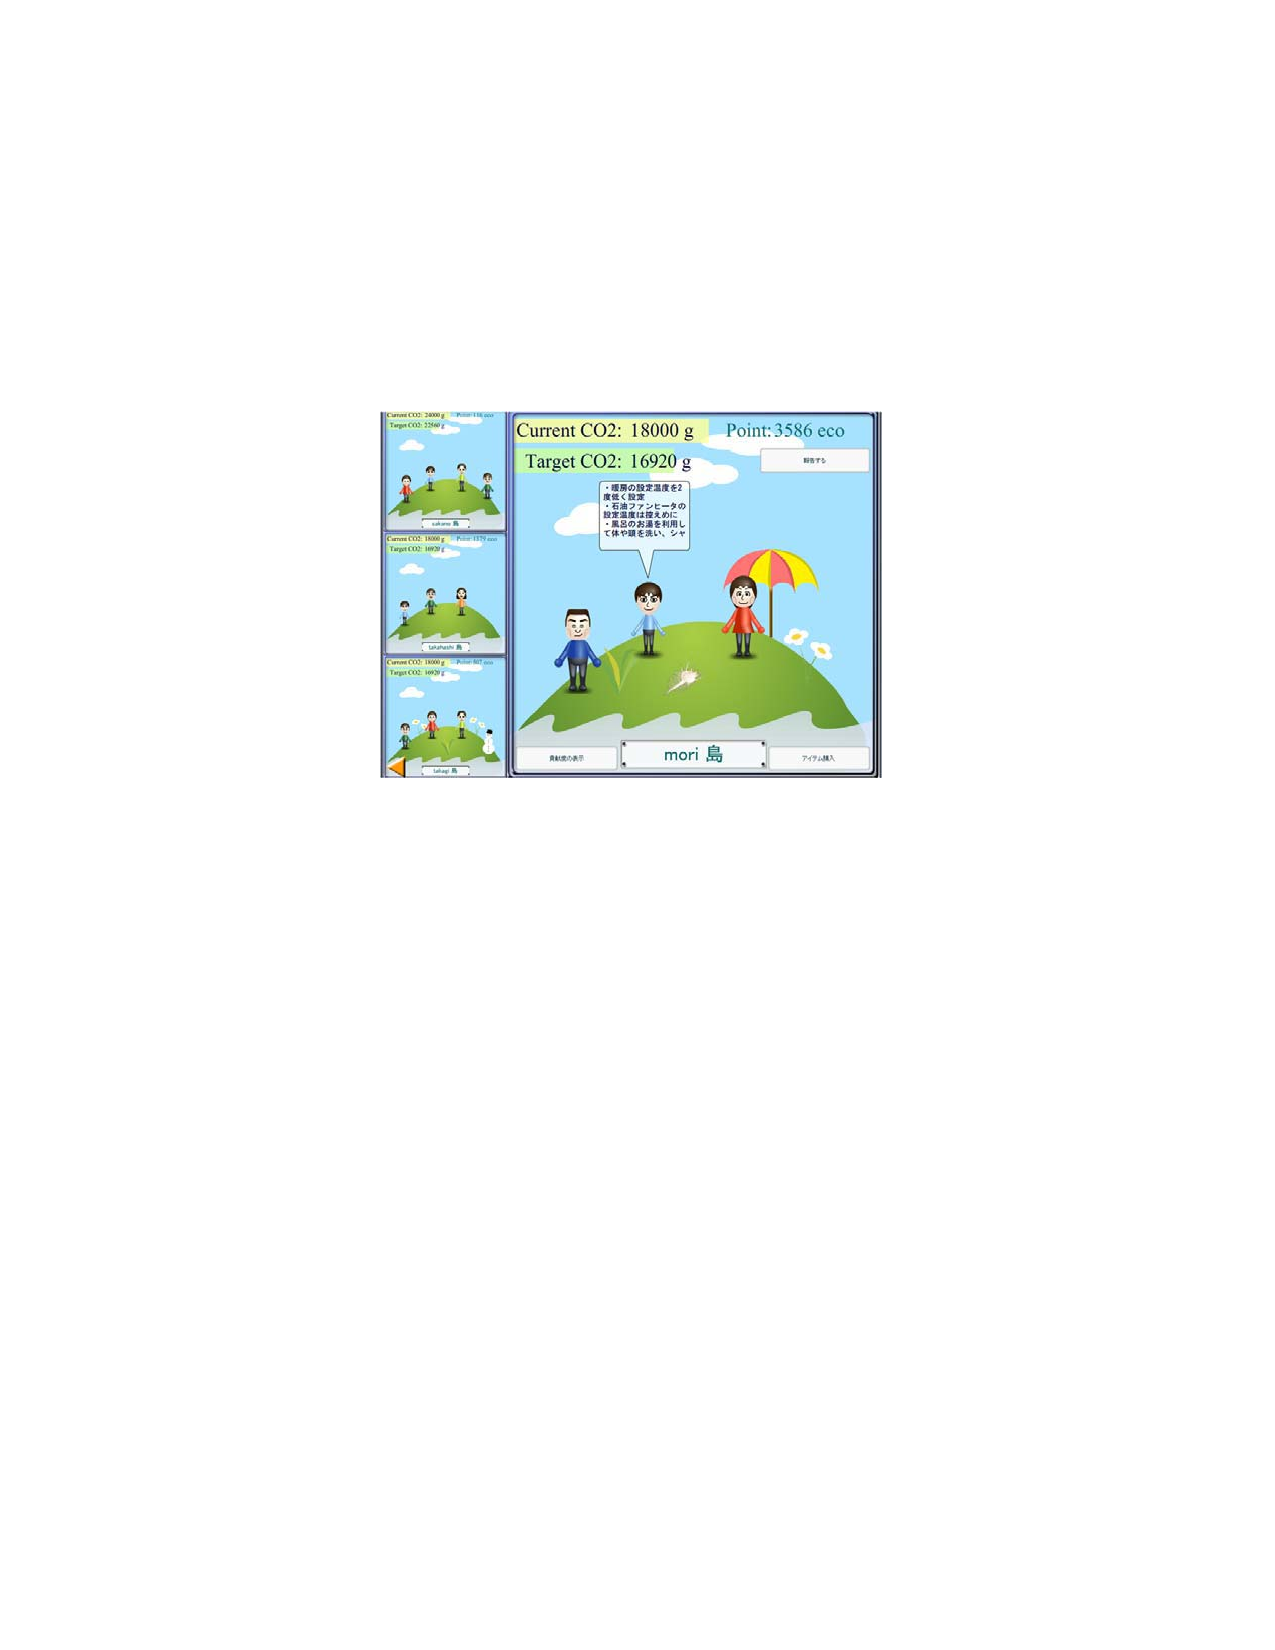
\includegraphics[width=0.8\textwidth]{ecoisland}
		\caption{Example EcoIsland display, with family avatars}
		\label{fig:ecoisland}
\end{figure}

Participants mobile phones have a list of suggested actions to reduce emissions, and they can self-report their actions using the phone. Participants can see the islands of other participants and they receive a periodic allowance in a virtual currency. The participants can use the virtual currency to buy decorations for their island, or to purchase carbon credits from other users. Participants with low emissions, therefore, can decorate their island, while those with high emissions have to spend their money on carbon credits. EcoIsland provides a metaphor for the users' emissions and makes them aware of the consequences of their actions.

The sensor portion of the system was not yet implemented at the time the authors conducted their study. The authors performed a four week pilot study of EcoIsland with 20 people in six families. During the first week, the baseline electricity usage of each participant's air conditioning system was monitored using a plug load meter (for more information on this type of meter, see \autoref{sec:plug-load-meters}). During the second week, one participant from each household was asked to use the system, while in the third week all members were asked to use it. In the fourth week, the carbon trading system was introduced to participants. At the conclusion of the study, the participants were surveyed and 17 of 20 participants said ``they were more conscious of environmental issues after the experiment than before.'' However, users indicated that they were motivated by game issues (such as saving the sinking island and buying decorations) rather than saving the environment. Few of the participants used the carbon trading system because their targets were easy enough to achieve without trading. Air conditioner usage in participant homes showed no correlation with game outcome, but the authors believe that the short study may have affected that outcome. The study was conducted in winter, which might seem like an inappropriate time to measure air conditioner use. However, in Japan, many air conditioning units also function as heaters, so it may be this type of air conditioner usage that the authors are referring to. One interesting result is that participants noted that manual reporting contributed to their motivation, so replacing the reporting with sensors could reduce user's motivation to change.

\subsection{Google PowerMeter}

\subsection{Microsoft Hohm}

\subsection{Virtual Polar Bear}

\subsection{iamgreen}

\section{Electricity Metering}

Electricity metering systems can be broken down into two types: plug load meters that measure the electrical load directly plugged into them, and whole home energy meters that measure the electrical usage of an entire home. Both typically provide a real-time display of electricity usage, and some sort of historical total (usually in kilowatt hours, kWh).

\subsection{Plug Load Meters}
\label{sec:plug-load-meters}

The Kill-A-Watt is an example of an inexpensive plug load meter \cite{kill-a-watt}. It is designed to be plugged into a wall outlet, and the load is then plugged into the Kill-A-Watt. An LCD display shows the current voltage, current, power, frequency, power factor, and cumulative energy used since the unit was plugged in. The Kill-A-Watt provides an easy way to determine how much electricity a particular appliance (or set of appliances if connected via a power strip) uses. The manufacturer claims the Kill-A-Watt has 0.2\% accuracy. There are several drawbacks to the Kill-A-Watt. Because of its shape, it generally obscures both of the outlets commonly found on a wall outlet in the US, preventing the second outlet from being use while measurement is taking place. The load must be plugged in via the Kill-A-Watt, so that means that the user must disconnect the load from power at least momentarily, which can be inconvenient for some loads (computers, refrigerators, etc.). The Kill-A-Watt also has no facility for exporting the data it collects, and if power is lost for any reason, the data collected will be lost as well. \fxnote{Add mention of newer model that stores data}

LeBlanc attempted to address the issue of data collection with his work on recording device-level power consumption \cite{leblanc-2007}. He developed a sensor that sits between the load and the wall outlet, like the Kill-A-Watt. The sensor records electricity usage, and transmits the data wirelessly using the ZigBee protocol to a base station. Details on how to construct the wireless power monitor can be found at the author's personal website \cite{LeBlanc2008power-mon-howto}. This system solves the problem of automated data collection, but still requires the load to be unplugged before monitoring. It also faces the problem of all plug-load meters, which is that it can only monitor what it is connected to, therefore it is unsuitable for providing a comprehensive picture of electricity usage in a home.

\fxnote{Need discussion of ACME meters here}

\subsection{Whole Home Meters}
\label{sec:whole-home-meters}

The Energy Detective TED Model 1001 is a whole home electricity meter from Energy, Inc \cite{the-energy-detective}. \fxnote{Need to update for TED 5000} TED consists of two portions: a base unit, which is connected directly to the incoming power lines at the circuit breaker box, and a display unit, which connects to any power outlet in the home. The base unit uses current transformers, which clamp over the incoming power cables, and measure the amount of current being transmitted over them. Because the transformers clamp over the existing cables, there is no need to alter the existing wiring. The instantaneous power consumption can be computed using the current data combined with the utility voltage. These data are transmitted to the display unit through the home's electrical wiring.

Once the display unit is plugged into any outlet in the home, it receives the instant power consumption data from the base unit once a second. The power consumption data can be displayed in real time in kW or dollars (after the user enters pricing data). It can also track historical consumption, peak usage, and project usage for the rest of the month based on historical usage. With the addition of the Footprints software package from Energy Inc, the display unit can be connected to a computer via USB to graph and record the data in a variety of formats. Energy Inc makes an API available for developers who wish to use the data directly. One developer has created an Open Source extension for the Firefox browser that displays electricity usage from TED in a toolbar inside Firefox \cite{Nick2008TED-the-Toolbar}. TED appears to be the lowest cost option for whole home electricity monitoring with computer data output.

While whole home energy meters provide only household-wide usage data, users can use the real-time display to figure out the impact of particular uses as air conditioning through trial and error experimentation. Parker et al.\ describe a protocol for using a household-wide meter and a circuit breaker panel to localize the energy usage in a home \cite{Parker2006How-Much-Energy}. All the breakers are turned off, and then turned on one at a time while recording data from the electrical meter. In 2--4 hours, users were able to generate a spreadsheet mapping the electricity usage in their homes.

\subsection{Building Energy Displays}
\label{sec:building-energy-displays}

Another type of electricity usage monitoring is building energy displays, which monitor electricity usage for an entire building (usually non-residential, like a school or office building) and display the usage information in some public area such as a lobby. Green TouchScreen \cite{greentouchscreen} and Building Dashboard \cite{building-dashboard} are examples of this type of product. These devices aim to make building occupants aware of the overall environmental impact of the building, which is something usually invisible to the occupants. Some systems make the displays available via the web so that users can view the information from their desk as well as the lobby. The displays often provide  information beyond just electricity usage, such as water or natural gas usage, and may display the usage in units other than kWh, such as number of incandescent light bulbs lit or hours of TV watching. Beyond their potential utility in helping building occupants to reduce their energy usage, informative displays can be used to get points toward Leadership in Energy and Environmental Design (LEED) certification for a building.

\section{Motivation and Persuasion}

\subsection{Public Commitments}

\subsection{Social Norms}

\subsection{Motives For Change}

\subsection{Design of Environmentally Persuasive Systems}


\section{Energy Literacy}
\label{sec:energy-literacy}

We believe energy literacy is critical to sustained positive environmental behavior change, so defining it and assessing it are critical.
